\documentclass{report}

\usepackage{amsfonts, amsmath, amssymb, amsthm}
\usepackage[margin=1.0in]{geometry}
\usepackage{hyperref}
\usepackage{float}
\usepackage{fancyhdr}
\usepackage{graphicx}
\usepackage[inkscapeformat=pdf]{svg}
\usepackage{mathrsfs}
\usepackage{comment}

\newcommand{\M}[2]{\mathbb{#1}^{#2}}
\newcommand{\twovector}[2]{\left[ \begin{array}{c} #1 \\ #2 \\ \end{array} \right]}
\newcommand{\threevector}[3]{\left[ \begin{array}{c} #1 \\ #2 \\ #3 \\ \end{array} \right]}
\newcommand{\fourvector}[4]{\left[ \begin{array}{c} #1 \\ #2 \\ #3 \\ #4 \\ \end{array} \right]}
\newcommand{\fivevector}[5]{\left[ \begin{array}{c} #1 \\ #2 \\ #3 \\ #4 \\ #5 \\ \end{array} \right]}
\newcommand{\sixvector}[6]{\left[ \begin{array}{c} #1 \\ #2 \\ #3 \\ #4 \\ #5 \\ #6 \\ \end{array} \right]}
\newcommand{\sevenvector}[7]{\left[ \begin{array}{c} #1 \\ #2 \\ #3 \\ #4 \\ #5 \\ #6 \\ #7 \\ \end{array} \right]}
\newcommand{\eightvector}[8]{\left[ \begin{array}{c} #1 \\ #2 \\ #3 \\ #4 \\ #5 \\ #6 \\ #7 \\ #8 \\ \end{array} \right]}
\newcommand{\ninevector}[9]{\left[ \begin{array}{c} #1 \\ #2 \\ #3 \\ #4 \\ #5 \\ #6 \\ #7 \\ #8 \\ #9 \\ \end{array} \right]}
\newcommand{\nbrack}[1]{\left( #1 \right)}
\newcommand{\bbrack}[1]{\left[ #1 \right]}
\newcommand{\cbrack}[1]{\left\lbrace #1 \right\rbrace}
\newcommand{\abrack}[1]{\left< #1 \right>}
\newcommand{\linebrack}[1]{\left| #1 \right|}
\newcommand{\twomatrix}[4]{\bbrack{
    \begin{array}{cc}
      #1 & #2 \\
      #3 & #4 \\
    \end{array}
  }
}
\newcommand{\threematrix}[9]{\bbrack{
    \begin{array}{ccc}
      #1 & #2 & #3 \\
      #4 & #5 & #6 \\
      #7 & #8 & #9 \\
    \end{array}
  }
}
\newcommand{\Lplc}[1]{\mathscr{L}\bbrack{ #1 } (s)}
\newcommand{\iLplc}[1]{\mathscr{L}^{-1}\bbrack{ #1 } (t)}
\newcommand{\til}[1]{\overset{~}{#1}}

\title{Innlevering 1}
\author{Jacob Oliver Bruun}
\date{\today}

\makeatletter
\let\inserttitle\@title
\let\insertauthor\@author
\makeatother

\pagestyle{fancy}
\chead{\insertauthor}
\lhead{\inserttitle}
\rhead{\today}

\parindent 0ex

\begin{document}


\section*{Oppg. 1}
Har 100 lodd med ett som gir $A$ og ett som gir $B$, ser at sjansen for at en ikke trekker loddet som gir $A$ er $99/100 \cdot 98/99 \cdot 97/98 \cdot 96/97$ og vi får da sannsynligheten for å trekke dette loddet
\begin{equation}
  \label{eq:1}
  P(A) = 1 - 99/100 \cdot 98/99 \cdot 97/98 \cdot 96/97 = \frac{4}{100}
\end{equation}
skal så finne $P(B|A)$ som er gitt ved
\begin{equation}
  \label{eq:2}
  P(B|A) = \frac{P(B \cap A)}{P(A)}
\end{equation}
det er fire muligheter for å få $A$ og i hver av de er det tre muligheter for å få $B$ og har dermed
\begin{equation}
  \label{eq:3}
  P(B\cap A) = \frac{4\cdot 3}{100\cdot 99\cdot 98\cdot 97}
\end{equation}
og har 12 forskjellige måter $A$ og $B$ kan trekkes og har dermed
\begin{equation}
  \label{eq:4}
  P(B\cap A) = \frac{12\cdot 98\cdot 97}{100\cdot 99\cdot 98\cdot 97}
\end{equation}
og kan finne
\begin{equation}
  \label{eq:5}
  P(B|A) = \frac{12\cdot 100\cdot 98\cdot 97}{4 \cdot 100\cdot 99\cdot 98\cdot 97} = \frac{1}{33}
\end{equation}
ser at det er $2\cdot 4\cdot 99\cdot 98\cdot 97 - 12\cdot 98\cdot 97$ forskjellige måter å trekke minstett av de to loddene, og vi vet det er $12\cdot 98\cdot 97$ mulige måter å trekke to av de og har dermed sannsynligheten
\begin{equation}
  \label{eq:11}
  P(A\land B | A\lor B) = \frac{12\cdot 98\cdot 97}{98\cdot 97 (8\cdot 99 - 12)} = \frac{1}{65}
\end{equation}


\section*{Oppg. 2}
Har oppgitt $P(A) = 0.2, P(B) = 0.5, P(A\cup B) = 0.6$. Dersom to hendelser ser disjunkte har vi at $P(A\cap B) = \emptyset$ dette vil føre til at $P(A) + P(B) = P(A\cup B)$ noe som ikke er tilfellet her og $A$ og $B$ er dermed ikke disjunkte. \\
For at hendelsene skal være uavhengige må vi ha $P(A|B) = P(A)$ kan bruke formelen fra \eqref{eq:2} og kan finne
\begin{equation}
  \label{eq:6}
  P(A\cap B) = P(A) + P(B) - P(A\cup B) = 0.1
\end{equation}
og kan da finne
\begin{equation}
  \label{eq:7}
  P(B|A) = \frac{0.1}{0.2} = 0.5 = P(B)
\end{equation}
og har dermed at $A$ og $B$ er uavhengige.


\section*{Oppg. 3}
\textbf{a)}
Har gitt $P(E) = 0.05, P(F) = 0.05, P(E\cap F) = 0.02$, har at
\begin{equation}
  \label{eq:8}
  P(R) = P(E\cup F) = P(E) + P(F) - P(E\cap F) = 0.08
\end{equation}
gjør samme analyse som tidligere
\begin{equation}
  \label{eq:9}
  P(E|F) = \frac{P(E\cap F)}{P(F)} = 0.40
\end{equation}
og ser dermed at $F$ og $E$ ikke er uavhengige hendelser, i tillegg er $P(E\cap F) \neq \emptyset$ og de er heller ikke disjunkte. \\

\textbf{b)}
Vet at $P(V | (E\cup F)') = 0.07, P(V | E\cup F) = 0.50$ og kan bruke
\begin{equation}
  \label{eq:18}
  P(V) = P(V|(E\cup F)')P((E\cup F)') + P(V| E\cup F)P(E\cup F) = 0.07\cdot 0.92 + 0.50\cdot 0.08 = 0.104
\end{equation}
ser så på
\begin{equation}
  \label{eq:19}
  \begin{split}
    P(E \cup F \cup V) &= P(E \cup F) + P(V) - P((E\cup F)\cap V) \\
                       &= P(E \cup F) + P(V) - P(V | E\cup F)P(E\cup F) \\
    &= 0.144
  \end{split}
\end{equation}


\section*{Oppg. 4}
Har følgende sannsynligheter $P(M) = 1/3, P(K) = 2/3, P(F|M) = 0.05, P(F|K) = 0.0025$ og skal finne $P(M|F)$, har fra \eqref{eq:2} en formel for sannsynligheten og vet at $P(M\cap F) = P(M)\cdot P(F|M)$ og $P(F) = 0.05/3 + 0.0025\cdot 2/3$
\begin{equation}
  \label{eq:10}
  P(M|F) = \frac{P(M\cap F)}{P(F)} = \frac{1/3 \cdot 0.05}{0.05/3 + 0.0025\cdot 2/3} = 0.90909
\end{equation}


\section*{Oppg. 5}
Ser på Morgans lover og ser først på $(A\cup B)'$ på venstre og $A' \cap B'$ på høyre
\begin{figure}[H]
  \centering
  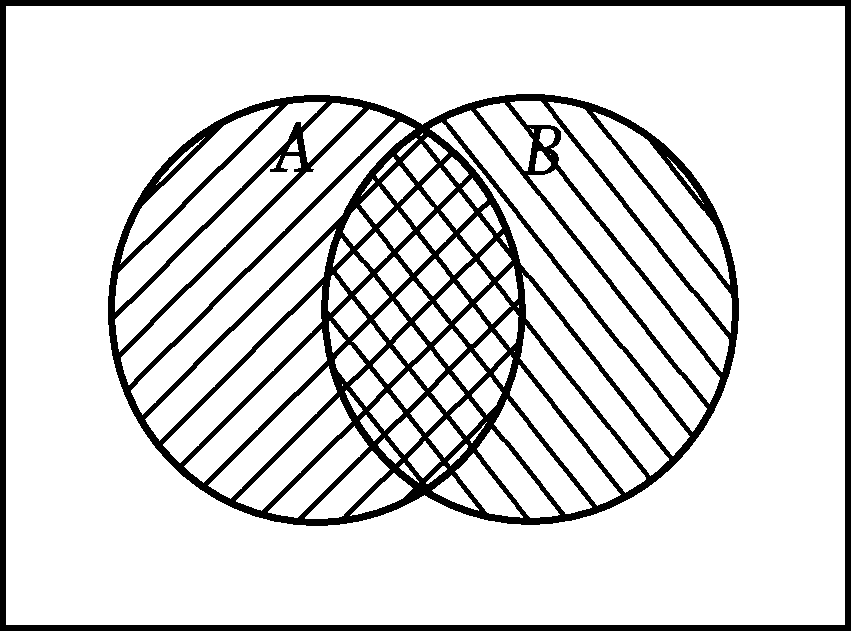
\includegraphics[width=0.3\textwidth]{pics/morgan_one.pdf} \;\;\;
  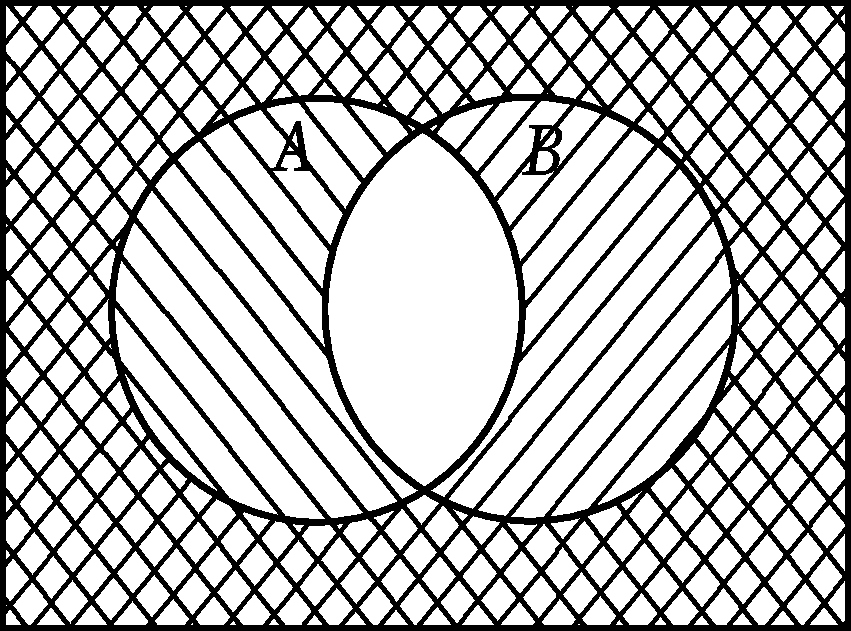
\includegraphics[width=0.3\textwidth]{pics/morgan_two.pdf}
\end{figure}
på venstre ser vi på komplementet av unionen og vil derfor se på alt som ikke er skrotet inn, mens på høyre ser vi på et snitt og dermed alt som har kryssete linjer og kan dermed se at $(A\cup B)' = A' \cap B'$. \\

Ser så på $(A\cap B)'$ på venstre og $A' \cup B'$ på høyre
\begin{figure}[H]
  \centering
  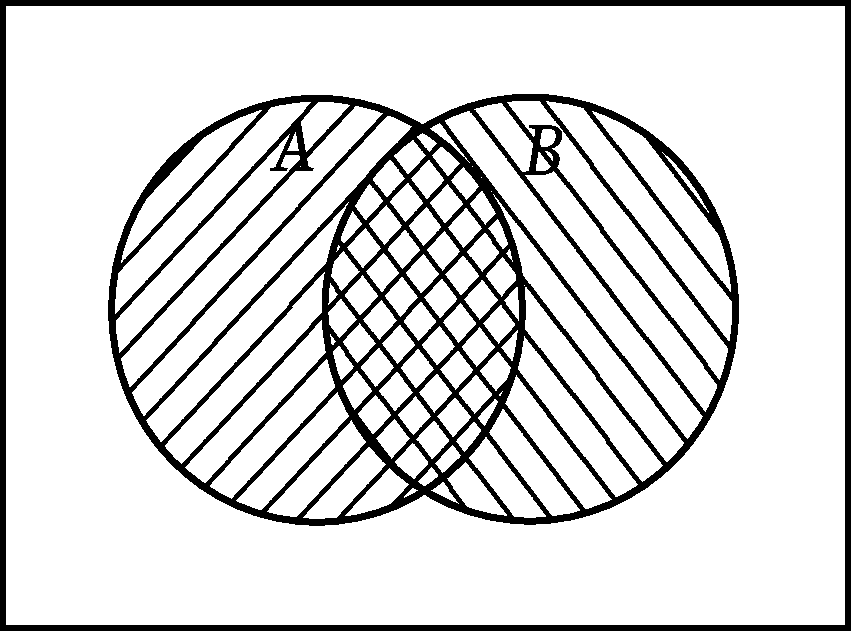
\includegraphics[width=0.3\textwidth]{pics/morgan_three.pdf} \;\;\;
  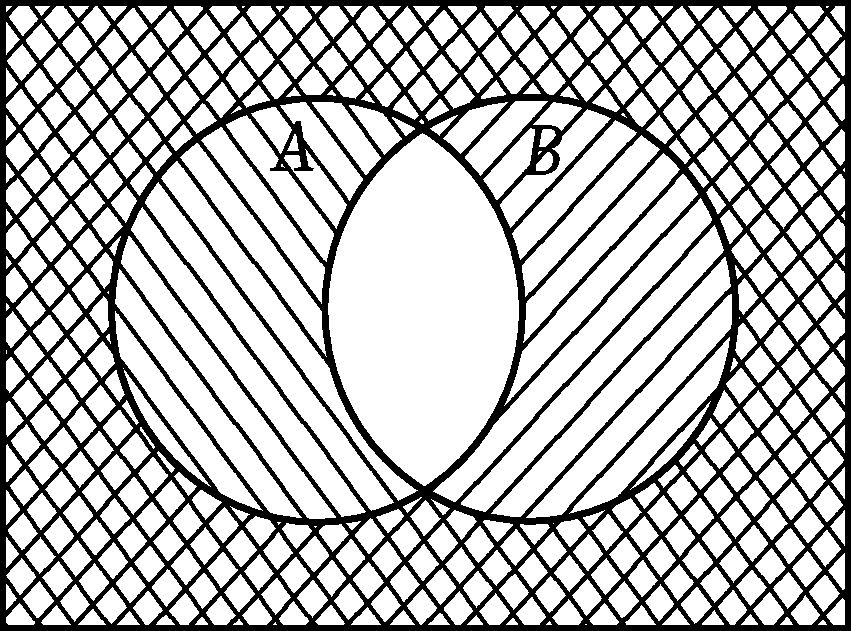
\includegraphics[width=0.3\textwidth]{pics/morgan_four.pdf}
\end{figure}
på venstre har vi komplementet av et snitt og ser dermed på alt som ikke har kryssete linjer og på høyre ser vi på unionen og dermed alt som er skrotet inn og kan dermed se at $(A\cap B)' = A' \cup B'$. \\


Ser på $A\cup (B\cup C)$ på venstre og $(A\cup B) \cup C$ på høyre
\begin{figure}[H]
  \centering
  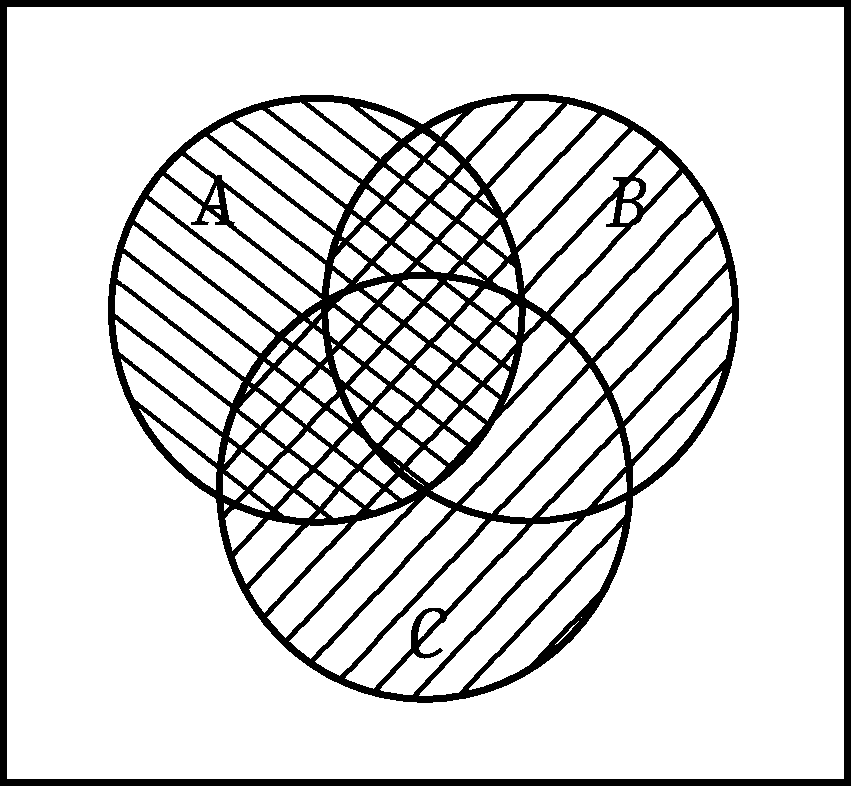
\includegraphics[width=0.3\textwidth]{pics/two.pdf} \;\;\;
  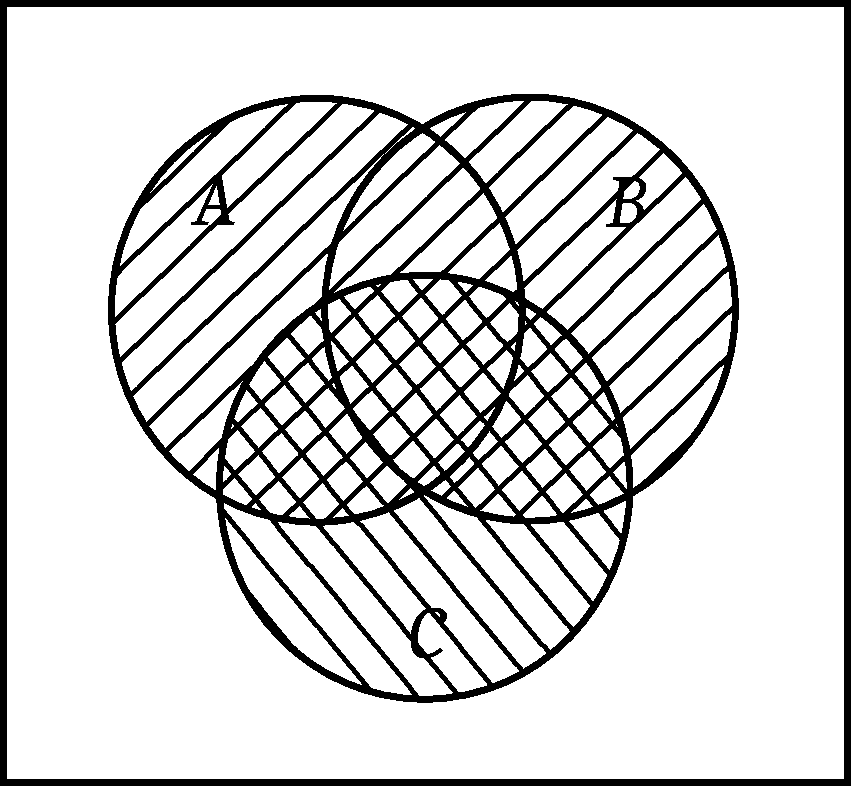
\includegraphics[width=0.3\textwidth]{pics/three.pdf}
\end{figure}
og dermed ser vi at $A\cup (B\cup C) = (A\cup B) \cup C$ siden de begge dekker alle tre sirklene. \\

Ser på $A\cap (B\cap C)$ på venstre og $(A\cap B) \cap C$ på høyre
\begin{figure}[H]
  \centering
  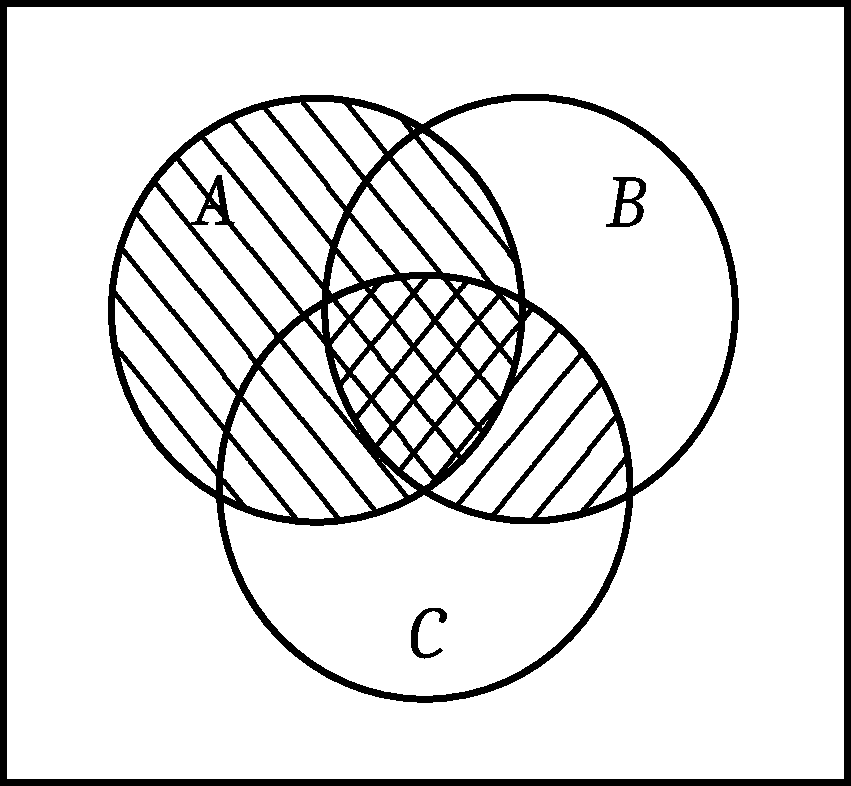
\includegraphics[width=0.3\textwidth]{pics/four.pdf} \;\;\;
  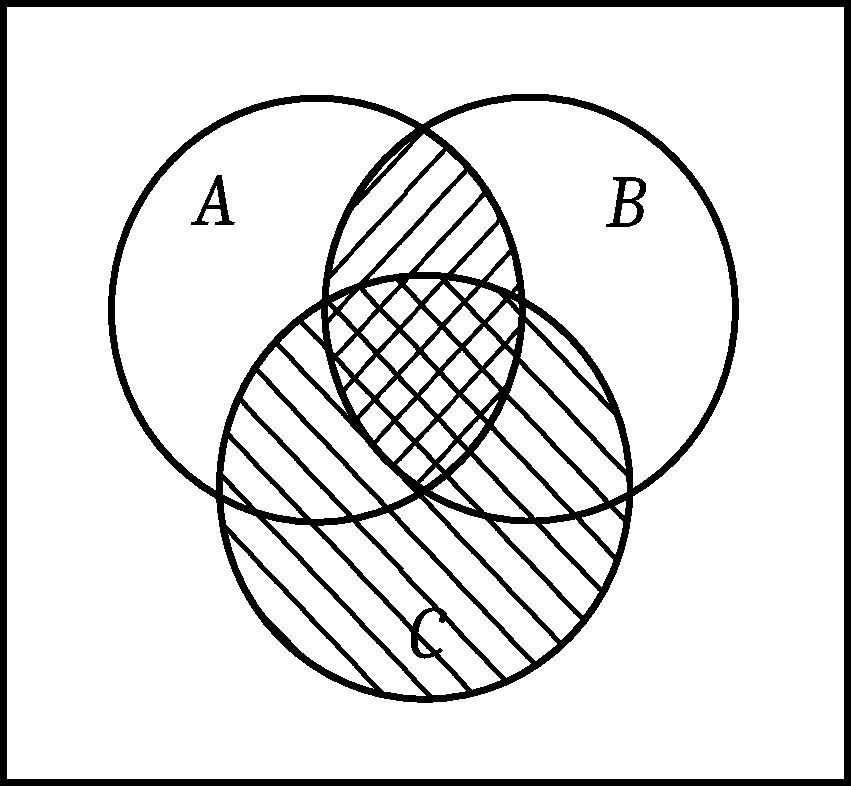
\includegraphics[width=0.3\textwidth]{pics/five.pdf}
\end{figure}
siden vi her ser på et snitt vil vi kun se der linjene krysser hverandre og disse områdene er like og dermed har vi $A\cap (B\cap C) = (A\cap B) \cap C$. \\

Ser på $A\cup (B\cap C)$ på venstre og $(A\cup B) \cap (A\cup C)$ på høyre
\begin{figure}[H]
  \centering
  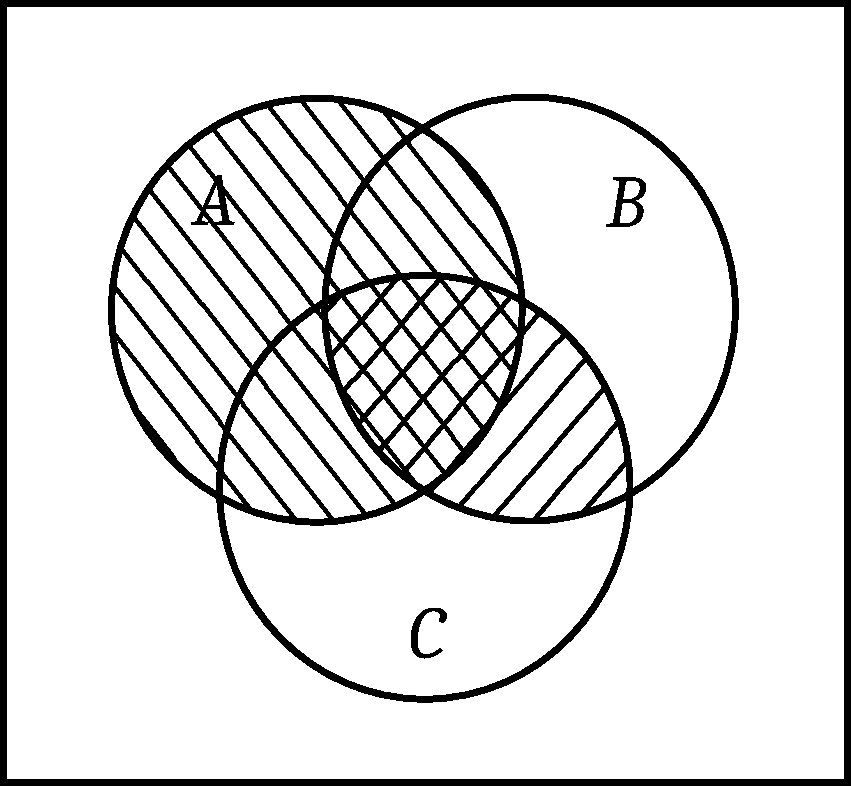
\includegraphics[width=0.3\textwidth]{pics/six.pdf} \;\;\;
  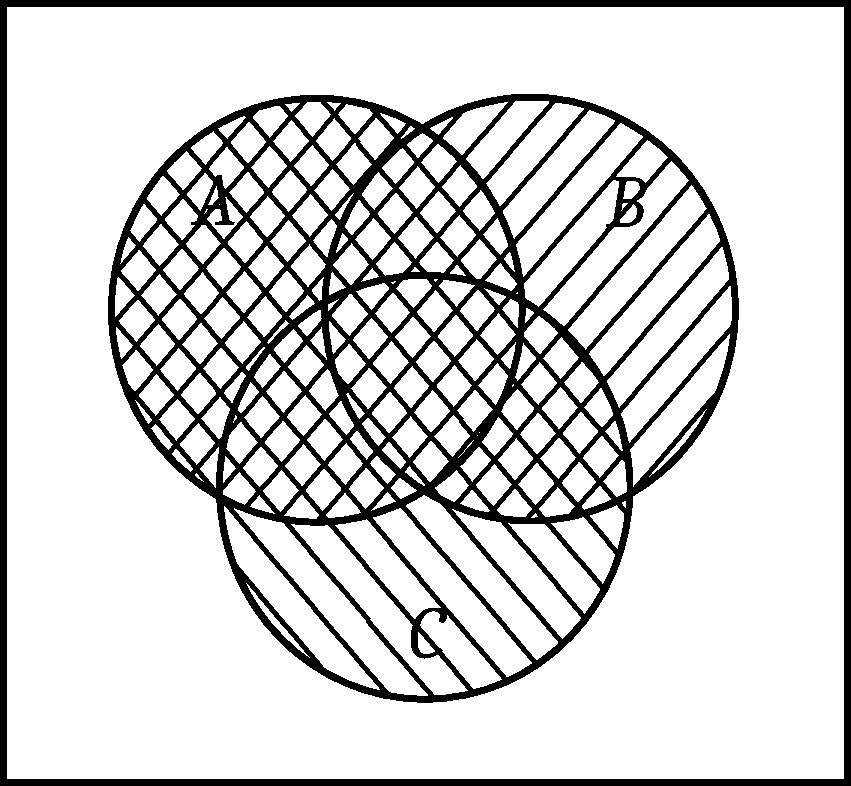
\includegraphics[width=0.3\textwidth]{pics/seven.pdf}
\end{figure}
på venstre ser vi på unionen og dermed alt som er skrotet inn, mens på høyre ser vi på snittet og dermed kun der vi har linjer som krysser hverandre og ser dermed at $A\cup (B\cap C) = (A\cup B) \cap (A\cup C)$. \\

Ser på $A\cap (B\cup C)$ på venstre og $(A\cap B) \cup (A\cap C)$ på høyre
\begin{figure}[H]
  \centering
  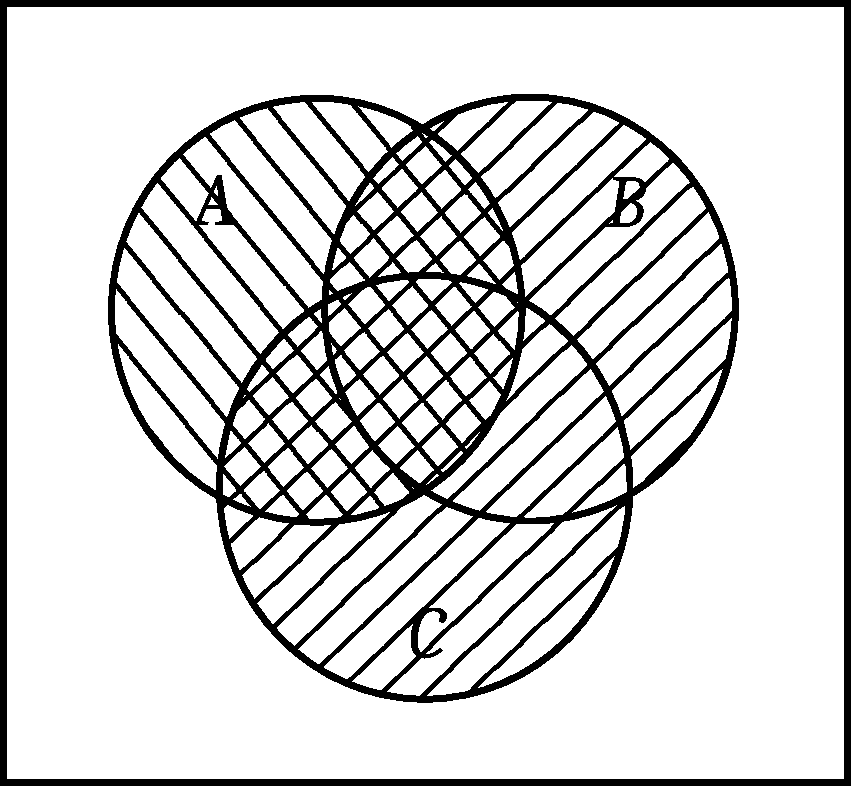
\includegraphics[width=0.3\textwidth]{pics/eight.pdf} \;\;\;
  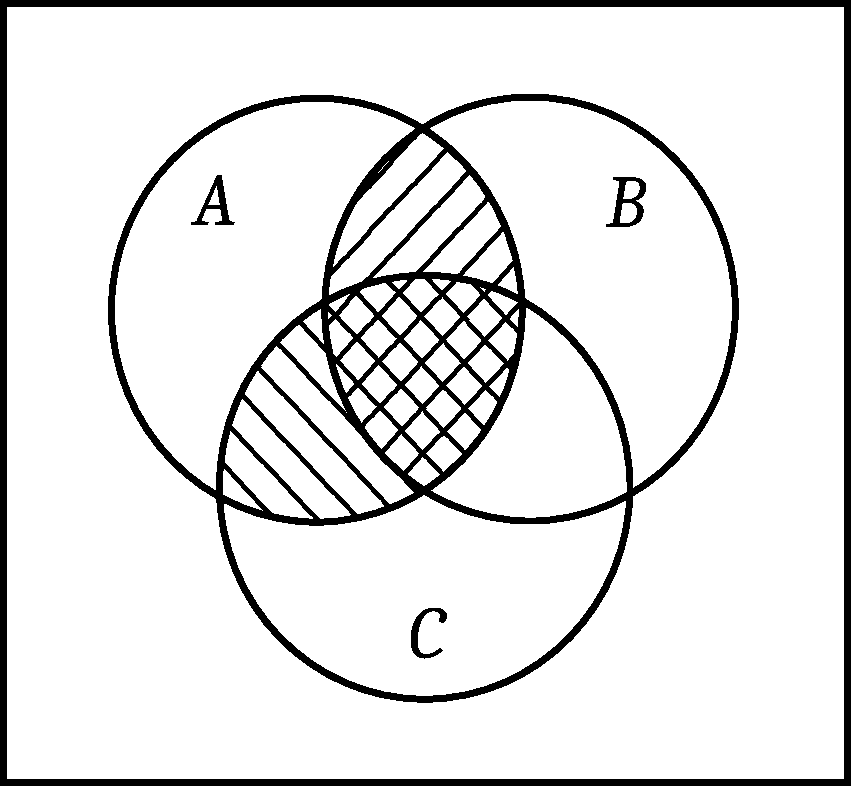
\includegraphics[width=0.3\textwidth]{pics/nine.pdf}
\end{figure}
ser da på området som er kryssete linjer på venstre og hele området som er skrotet inn på høyre og har dermed $A\cap (B\cup C) = (A\cap B) \cup (A\cap C)$.



\section*{Oppg. 6}
\textbf{a)}
Har fått oppgitt at $P(D) = 0.003$ og at $P(A|D) = 0.99$ og kan dermed finne forventet antall voksne nordmenn med sykdommen
\begin{equation}
  \label{eq:12}
  P(D) \cdot 3 000 000 = 9000
\end{equation}
og en vil forvente at prøven ikke slår ut for
\begin{equation}
  \label{eq:13}
  9000 \cdot \nbrack{ 1 - P(A|D) } = 90.
\end{equation}

\textbf{b)}
Skal finne $P(D' | A)$ og vet ved Bayes regel at
\begin{equation}
  \label{eq:14}
  P(D'|A) = \frac{ P(A | D')P(D') }{P(A)} = \frac{ P(A | D')P(D') }{P(A|D)P(D) + P(A|D')P(D')} = 0.6266
\end{equation}
ser så på
\begin{equation}
  \label{eq:17}
  P(D|A') = \frac{P(A'|D) P(D)}{P(A')} = \frac{P(A'|D) P(D)}{P(A'|D')P(D') + P(A'|D)P(D)} = 3.02\cdot 10^{-5}
\end{equation}
ser dermed at det er stor sannsynlighet for at det er en falsk positiv når det er få som har sykdommen, og at det er svært liten sjanse for at du har sykdommen dersom du tester negativt.


\end{document}
